\documentclass{article}
    % General document formatting
    \usepackage[margin=1in]{geometry}
    \usepackage[parfill]{parskip}
    \usepackage[utf8]{inputenc}
    \usepackage{amsmath}

    % Additional packages required
    \usepackage{multirow}
    \usepackage{fancyhdr}
    \usepackage{setspace}
    \usepackage{marginnote}
    \usepackage{graphicx}
    \usepackage{vhistory}
    \usepackage{amssymb} % for \therefore

    % Don't ever hypenate words
    \hyphenpenalty=10000
    \exhyphenpenalty=10000

    % Pull images from ./images/
    \graphicspath{ {images/} }

% General document setup
\pagenumbering{gobble}
\title{Previously Derived Equations}
\author{Engr 16x Teaching Team}

% Line spacing
\onehalfspacing

% Page headers/footers
\pagestyle{fancy}
\fancyhf{}
\rhead{Previously Derived Equations}
\lhead{ENGR 16100}
\cfoot{\textbf{Note: You will \underline{not} have access to these derivations during any exam.} \\ \textit{All rights reserved by Purdue University, \the\year. Last revised \today.}}

% Some nice looking coordinate symbols
\newcommand{\ihat}{\hat{\textbf{\i}}}
\newcommand{\jhat}{\hat{\textbf{\j}}}
\newcommand{\erhat}{\hat{\textbf{e}}_\textbf{r}}
\newcommand{\ethat}{\hat{\textbf{e}}_\textbf{$\theta$}}

\begin{document}

%------------------------------------------------
%	Title Page
%------------------------------------------------
\begin{titlepage} % Suppresses headers and footers on the title page
    
    \centering % Centre everything on the title page
    
    \scshape % Use small caps for all text on the title page
    
    \vspace*{\baselineskip} % White space at the top of the page
    
    %------------------------------------------------
    %	Title
    %------------------------------------------------
    
    \rule{\textwidth}{1.6pt}\vspace*{-\baselineskip}\vspace*{2pt} % Thick horizontal rule
    \rule{\textwidth}{0.4pt} % Thin horizontal rule
    
    \vspace{0.75\baselineskip} % Whitespace above the title
    
    {\LARGE ENGR 16100\\ Previously Derived Equations\\} % Title
    
    \vspace{0.75\baselineskip} % Whitespace below the title
    
    \rule{\textwidth}{0.4pt}\vspace*{-\baselineskip}\vspace{3.2pt} % Thin horizontal rule
    \rule{\textwidth}{1.6pt} % Thick horizontal rule
    
    \vspace{2\baselineskip} % Whitespace after the title block
    
    %------------------------------------------------
    %	Subtitle
    %------------------------------------------------
    
    A Useful Set of Equations Discussed in Lecture  % Subtitle or further description
    
    \vspace*{3\baselineskip} % Whitespace under the subtitle
    
    %------------------------------------------------
    %	Editor(s)
    %------------------------------------------------
    
    Edited By
    
    \vspace{0.5\baselineskip} % Whitespace before the editors
    
    {\scshape\Large Eric Nauman \\ Tim Whalen \\ Nicky Marino \\} % Editor list
    
    \vspace{0.5\baselineskip} % Whitespace below the editor list
    
    \textit{Purdue University \\ West Lafayette, IN} % Editor affiliation
    
    \vfill % Whitespace between editor names and publisher logo
    
    %------------------------------------------------
    %	Footer
    %------------------------------------------------
    
    \vspace{1\baselineskip}
    
    \textbf{Note: You will \underline{not} have access to these derivations during any exam.}

\end{titlepage}

%------------------------------------------------
%	General Derivations
%------------------------------------------------

\section*{General Derivations}

\textbf{Newton's Second Law} \\
$\sum \vec{F} = m \vec{a}$ \\

\textbf{Kinematics} \\
\begin{tabular} {@{} ll }
    Cartesian                                                       & Polar \\
    $\vec{r} = x\ihat + y\jhat + z\hat{k}$                      & $\vec{r} = r\erhat$ \\
    $\vec{v} = \dot{x}\ihat + \dot{y}\jhat + \dot{z}\hat{k}$    & $\vec{v} = \dot{r}\erhat + r\dot{\theta}\ethat$ \\
    $\vec{a} = \ddot{x}\ihat + \ddot{y}\jhat + \ddot{z}\hat{k}$ & $\vec{a} = (\ddot{r} - r\dot{\theta}^2) \erhat + (r\ddot{\theta} + 2\dot{r}\dot{\theta})\ethat$
\end{tabular} \\

$\vec{p} = m \vec{v}$ \\
$\Delta \vec{p} = \int\vec{F}dt$ \\

\textbf{Universal Accounting Equation} \\
$(\text{Final value} - \text{Initial value}) = (\text{Input} - \text{Output}) + (\text{Generated} - \text{Consumed})$ \\

\textbf{Energies} \\
Gravitational Potential: $E_g = mgh$ \\
Elastic Potential: $E_{sp} = \frac{1}{2} k (\Delta x)^2$ \\
Kinetic: $E_k = \frac{1}{2}mv^2$ \\

\clearpage

%------------------------------------------------
%	Impulse-Momentum Equation
%------------------------------------------------

\section*{Linear Impulse-Momentum Equations}
Single Particle:
\begin{align*}
    \Delta\vec{p} &= \int_{t_{state 1}}^{t_{state 2}} \vec{F}_{net} dt  \\
                  &= m\vec{v}_2 - m\vec{v}_1
\end{align*}

System of Particles: 
\begin{align*}
    \Delta\vec{p}_{total} &= \int_{t_{state 1}}^{t_{state 2}} \vec{F}_{net}^{ext} \\
                          &= \sum_i \left( m_i\vec{v}_{i, state 2} - m_i\vec{v}_{i, state 1} \right)
\end{align*}

Conservation of Momentum:
\begin{align*}
    0 &= \sum_i \left( m_i\vec{v}_{i, state 2} - m_i\vec{v}_{i, state 1} \right) \\
      &= \sum_i m_i\vec{v}_{i, state 2} - \sum_i m_i\vec{v}_{i, state 1} \\
    \sum_i m_i\vec{v}_{i, state 1} &= \sum_i m_i\vec{v}_{i, state 2}
\end{align*}

\clearpage

%------------------------------------------------
%	Direct and Oblique Impact
%------------------------------------------------

\section*{Direct and Oblique Impact}

\textbf{Motion in a Normal Direction} \\
Motion in a normal direction looks exactly the same as a direct impact. Thus, the motion can be described using the Conservation of Momentum and the Coefficient of Restitution equations:
\begin{equation*}
    m_A \left(v_{A, n} \right)_1 + m_B \left( v_{B, n} \right)_1 = m_A \left(v_{A, n} \right)_2 + m_B \left( v_{B, n} \right)_2
\end{equation*}
\begin{equation*}
    e = -\frac{\left(v_{A, n} \right)_2 - \left( v_{B, n} \right)_2}{\left(v_{A, n} \right)_1 - \left( v_{B, n} \right)_1}
\end{equation*} \\

\textbf{Motion in a Tangent Direction} \\
Motion in a tangent direction does not result in any changes in velocity:
\begin{align*}
    \left(v_{A, t} \right)_1 &= \left(v_{A, t} \right)_2 \\
    \left(v_{B, t} \right)_1 &= \left(v_{B, t} \right)_2
\end{align*}

\textbf{Note:} For direct impact problems, you should only use the "motion in a normal direction" equations.

\clearpage

%------------------------------------------------
%	Angular Momentum
%------------------------------------------------

\section*{Angular Momentum}

The formal definition of the angular momentum $\vec{L}_Q$ of a particle about a point $Q$ is:
\begin{align*}
    \vec{L}_Q &= \vec{r}_Q \times \left( m \vec{v} \right) \\
              &= \vec{r}_Q \times \vec{p}
\end{align*}
where $\vec{r}_Q$ is the position vector of the particle measured from point $Q$.

\begin{figure}[h]
    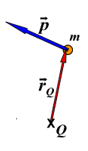
\includegraphics[scale=0.7]{angular_momentum_no_text}
    \centering
\end{figure}

\clearpage

%------------------------------------------------
%	Kinetic Energy
%------------------------------------------------

\section*{Kinetic Energy}

You all know Newton's Second Law: \\
\begin{equation*}
    \Sigma \vec{F} = m \vec{a}
\end{equation*}

We can use this equation to find power using kinetic energy $T$:
\begin{align*}
    T &= \frac{1}{2}m\vec{v} \cdot \vec{v} \\
    \frac{dT}{dt}         &= \frac{1}{2}m\vec{a} \cdot \vec{v} + \frac{1}{2}m\vec{v} \cdot \vec{a} \\
                          &= \frac{1}{2}m\vec{a} \cdot \vec{v} + \frac{1}{2}m\vec{a} \cdot \vec{v} \\
                          &= m \vec{a} \cdot \vec{v} \\
                          &= \left( \Sigma \vec{F} \right) \cdot \vec{v} \\
                          &= \text{Power}
\end{align*}

That's a nice result, but what if we integrate both sides?
\begin{align*}
    \int_{t_1}^{t_2} \left(\frac{dT}{dt} \right) dt &= \int_{t_1}^{t_2} \left( \Sigma \vec{F} \cdot \vec{v} \right) dt \\
    \int_{T_1}^{T_2} dT                             &= \int_{t_1}^{t_2} \left( \Sigma \vec{F} \cdot \frac{d\vec{r}}{dt} \right) dt \\
    T_2 - T_1                                       &= \int_{\vec{r}_1}^{\vec{r}_2} \Sigma \vec{F} \cdot d\vec{r}   \hspace{0.2cm} \text{\footnotemark} \\
    T_2 - T_1                                       &= \int_{S_1}^{S_2} \left( \Sigma \vec{F} \right) \cdot \hat{e}_t ds \hspace{0.15cm} \text{\footnotemark} \\
    \Delta T                                        &= \frac{1}{2} m \left( \vec{v}_2 \cdot \vec{v}_2 \right) - \frac{1}{2} m \left( \vec{v}_1 \cdot \vec{v}_1 \right)
\end{align*}

\addtocounter{footnote}{-1}
\footnotetext{Since this is a dot product, we can replace $d\vec{r}$ with the tangent---the arc length along the particle's path.}
\stepcounter{footnote} \footnotetext{This is equal to the work done on the particle.}

\begin{figure}[h]
    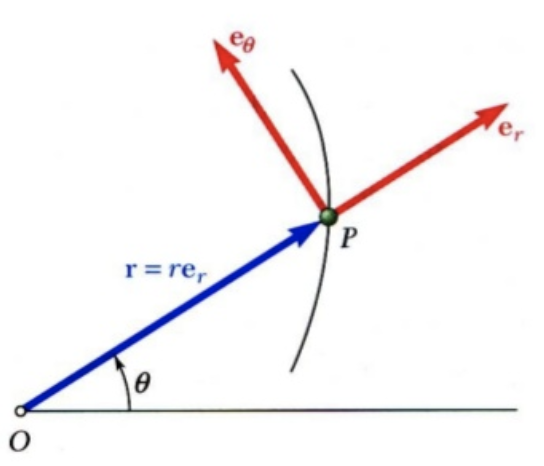
\includegraphics[scale=0.7]{img1}
    \centering
\end{figure}

\clearpage

%------------------------------------------------
%	Cartesian and Polar Coordinates
%------------------------------------------------

\section*{Cartesian and Polar Coordinates}

Start with the position vector:
$$\vec{r} = x\ihat + y\jhat$$

Using the Chain Rule, the derivative of $\vec{r}$ is
$$\vec{v} = \frac{dx}{dt}\ihat + x\frac{d\ihat}{dt} + \frac{dy}{dt}\jhat + y\frac{d\jhat}{dt}$$

Because unit vectors in Cartesian coordinates are fixed and constant, $\frac{d\ihat}{dt} = \frac{d\jhat}{dt} = \vec{0}$, so we can rewrite velocity as
\begin{align*}
    \vec{v} &= \frac{dx}{dt}\ihat + \frac{dy}{dt}\jhat \\
            &= \dot{x}\ihat + \dot{y}\jhat \hspace{0.2cm} \text{\footnotemark} \\
    \vec{a} &= \ddot{x}\ihat + \ddot{y}\jhat
\end{align*}

\stepcounter{footnote} \footnotetext{Note that $\dot{x} = \frac{dx}{dt}$}

We can also describe the motion of the particle using polar coordinates:
\begin{align*}
    \vec{r} &= r\erhat \\
    \vec{v} &= \dot{r}\erhat + r \frac{d\erhat}{dt}
\end{align*}

Before continuing, we need to work out the derivatives of the following equations:
\begin{align*}
    \erhat &= \ihat \cos\theta + \jhat \sin\theta \\
    \ethat &= -\ihat \sin\theta + \jhat \cos\theta
\end{align*}

The trick is to use the Chain Rule to find their derivatives:
\begin{align*}
    \frac{d\erhat}{dt} &= \frac{d\erhat}{d\theta} \cdot \frac{d\theta}{dt} \\
                       &= \frac{d\erhat}{d\theta} \dot{\theta} \\
                       &= \left( -\ihat\sin\theta + \jhat\cos\theta \right) \dot{\theta} \\
                       &= \dot{\theta} \ethat \\ \\
    \frac{d\ethat}{dt} &= \frac{d\ethat}{d\theta} \cdot \frac{d\theta}{dt} \\
                       &= \dot{\theta} \left[ -\ihat\cos\theta -\jhat\sin\theta \right] \\
                       &= \dot{\theta} \left( -\erhat \right) \\
                       &= -\dot{\theta} \erhat
\end{align*}

Combining the above derivatives into our equation for velocity, we get
\begin{align*}
    \vec{v} &= \dot{r} \erhat + r \left( \dot{\theta} \ethat \right) \\
            &= \dot{r} \erhat + r \dot{\theta} \ethat \\ \\
    \vec{a} &= \ddot{r} \erhat + \dot{r} \frac{d\erhat}{dt} + \dot{r} \left( \dot{\theta} \ethat \right) + r \ddot{\theta} \ethat + r \dot{\theta} \frac{d\ethat}{dt} \\
            &= \ddot{r} \erhat + \dot{r} \dot{\theta} \ethat + \dot{r} \dot{\theta} \ethat + r \ddot{\theta} \erhat - r \dot{\theta}^2 \erhat \\
            &= \left( \ddot{r} - r \dot{\theta}^2 \right) \erhat + \left( r \ddot{\theta} + 2\dot{r}\dot{\theta} \right) \ethat
\end{align*}

\begin{figure}[h]
    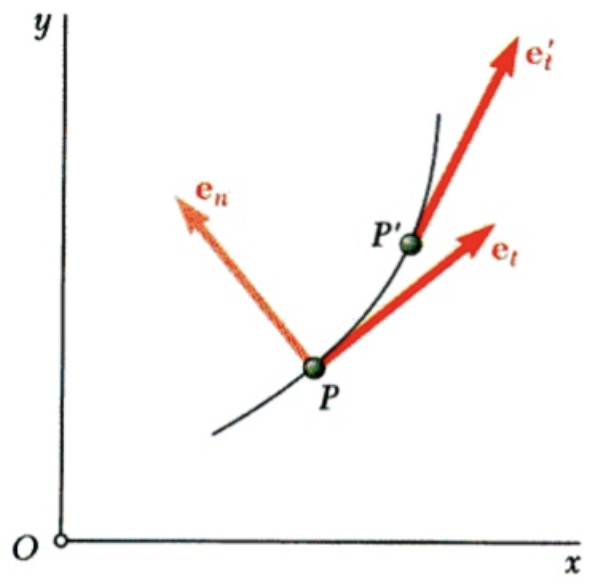
\includegraphics[scale=0.7]{img2}
    \centering
\end{figure}

%------------------------------------------------
%	Version History
%------------------------------------------------
\clearpage
\begin{versionhistory}
    \vhEntry{1.0}{11/26/17}{NSM}{Creation}
    \vhEntry{1.1}{12/2/17}{NSM}{Fixed typo in \textit{Motion in a Tangent Direction}}
\end{versionhistory}

\end{document}